\documentclass[sans, aspectratio=169]{beamer}
%\usepackage{eulervm}
\usepackage[scaled ]{helvet}
\usepackage[utf8]{inputenc}
\usepackage{multimedia}

\usepackage[T1]{fontenc}

\title{\textbf{{\LARGE  Plasma for space exploration}}\\
On the Hall Effect Thruster investigation}
\date[JS-EDOM2018]{Journées scientifiques de l'EDOM - 15/02/2018}
\author[A. Tavant]{Antoine Tavant}

%\usetheme{LPP}
\usepackage{template/beamerthemeLPP}
\begin{document}

\begin{frame}
\titlepage
\end{frame}

\begin{frame} 
	\frametitle{Propulsion for satellites} 
	\framesubtitle{Introduction} 
	\vspace{-1.07cm}
	\begin{columns}
		\begin{column}{0.75\linewidth}
		
			\begin{itemize} 
				\item Satellites are increasingly used/needed
				
				\begin{figure}[hbtp]
				\centering
				\includegraphics[scale=0.3]{images/sattelite-number.jpg}
				\caption{Number of small satellite launched [IDSA, 2016]}
			\end{figure}
			
				\item Propulsion is key : life time, capability, performances, etc. 

			\end{itemize}
					
		\end{column}
		
		\begin{column}{0.3\linewidth}
		
			\begin{flushright}
			\includegraphics[scale=0.3]{images/arian5.jpg} 
			\end{flushright}
			
		\end{column}
		
	\end{columns}
	
\end{frame}

\begin{frame} 
	\frametitle{The Hall effect Thruster} 
	\framesubtitle{Introduction} 
	\begin{itemize} 
		\item Efficiency of a thruster is linked to the exhaust velocity. To send $10^4 kg$ to Mars:
		
		%\vspace{0.2cm}
		\renewcommand{\arraystretch}{1.2}% Wider
		\begin{center}
			\begin{tabular}{l|c|c|c}
				Technology & Exhaust velocity $/km.s^{-1}$ &Properllant mass $/10^3kg$\\ \hline 
				Chemical & $1 $ &     $190$   \\
				Electrical & $10$&   $3.5$ 
			\end{tabular}
		\end{center}
		\pause
		\vspace{0.2cm}
		\item Hall Effect Thrusters (HET) is a very promissing electrical technology :
		\begin{itemize} 
			\item High exhaust velocity ($\sim 12 km/s$)
			\item \textit{Smart1} spacecraft used it \textbf{to fly to the moon} [ESA, 2009]
			\item Selected for \textbf{human missons to Mars} ! [NASA, 2017]
		\end{itemize}
	\end{itemize}
		
\end{frame}


\begin{frame} 
	\frametitle{The Hall effect Thruster} 
	\framesubtitle{More details} 

\begin{columns}

	\begin{column}{0.45\linewidth}
		\begin{figure}[hbtp]
		\centering
		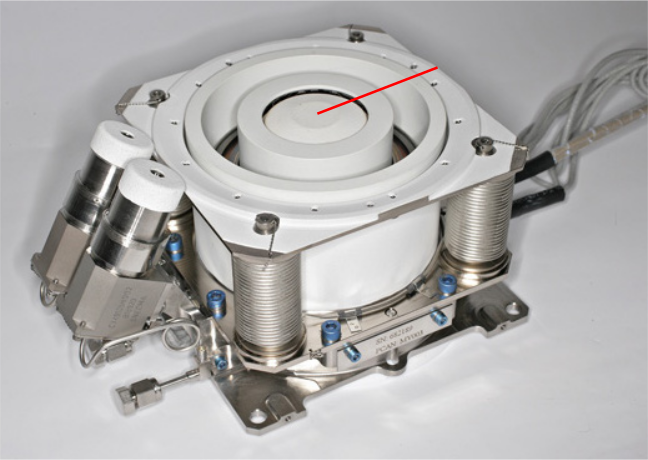
\includegraphics[scale=0.25]{images/PPS1350-G.png}
		\caption{HET (PPS-1350, Safran )}
		\end{figure}
	
	\end{column}

	\begin{column}{0.45\linewidth}
		\begin{figure}[hbtp]
		\centering
		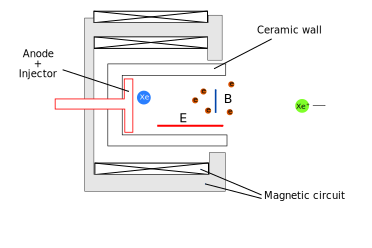
\includegraphics[scale=0.7]{images/HET.png}
		\caption{Shematic cut of an HET}
		\end{figure}
	
	\end{column}

\end{columns}	
\pause
\begin{center}
	(Un)fortunately: \textbf{the HET is still poorly understood}

\end{center}
\end{frame}

\begin{frame} 
\frametitle{What don't we know ?} 
\framesubtitle{Introduction} 
Better inderstanding of HET is important:

\begin{itemize}
\item Performance (thrust, efficentcy, etc.) isn't predictable:
	\begin{itemize}
		\item the electron axial mobility is anormaliously high ($\sim 10 \times$)
		\item the wall effect is poorly understood
	\end{itemize}
\item The life time isn't predictable
	\begin{itemize}
		\item Walls are eroded by ion impact sputtering
		\item Life time up to 7000h
	\end{itemize}
\end{itemize}

\begin{center}
\textbf{Why ?} \pause Because plasma physics are \textbf{difficult}

\end{center}
\end{frame}

\begin{frame}{Plasma physics are \textbf{difficult}} 

	\begin{itemize}
	\item Measurments and diagnotics are difficult:
		\begin{itemize}
			\item Intrusive probs will modify the plasma properties
			\item Non-intrusive diagnostics are costly, complicated, and work badly under these conditions
		
		\end{itemize}
	\end{itemize}
	\begin{itemize}
	\item The therory is complexe:
		\begin{itemize}
			\item Plasma : \textbf{fluid equations} mixed with \textbf{Maxwell equations} $\rightarrow$ quite complex
		
		\end{itemize}
	\end{itemize}
	$\rightarrow$ Simulation is a big help, especially kinetic simulations.
\end{frame}


\begin{frame}
	\frametitle{Plasma Beam Instability} 
	\framesubtitle{Some Plasma Physics} 

	An example of "simple" plasma behavious : the 1D plasma-beam instability.

\begin{columns}

\begin{column}{0.55\linewidth}
The system is simple:
	\begin{itemize}
		\item a static plasma background
		\item an electron beam with high velocity
		\item collisions are neglected (low pressure)
		\item uniform spatial density
	\end{itemize}
\end{column}

\begin{column}{0.35\linewidth}

\includegraphics<1>[scale=0.4]{images/plasma_beam_f_v.png} 

\end{column}

\end{columns}	

\end{frame}

\begin{frame}
	\frametitle{Plasma Beam Instability} 
	\framesubtitle{Some Plasma Physics} 

	An example of "simple" plasma behavious : the 1D plasma-beam instability.

\begin{columns}

\begin{column}{0.55\linewidth}
The system is simple:
	\begin{itemize}
		\item a static plasma background
		\item an electron beam with high velocity
		\item collisions are neglected (low pressure)
		\item uniform density
		
	\end{itemize}
\end{column}

\begin{column}{0.35\linewidth}
\begin{tiny}
\vspace{0.05cm}

	Phase-space representation of electrons \\ (Velocity vs position)
	\movie[width=5cm,height=4.18cm,poster,showcontrols=false,autostart]{}{images/BeamInstability.mp4}
\end{tiny}

\end{column}

\end{columns}	

\end{frame}




\begin{frame} 
	\frametitle{Simulation of HET} 
	\framesubtitle{ Investigating the ECDI } 
	Research done at LPP: 
	2D simulation of HET with LPPic, a PIC simulation tool
	\begin{columns}

	\begin{column}{0.45\linewidth}
		\begin{figure}[hbtp]
		\centering
		\includegraphics[scale=0.25]{images/Simulationcut.png}
	\end{figure}
	
	\end{column}

	\begin{column}{0.45\linewidth}
		\begin{figure}[hbtp]
		\centering
		\includegraphics[scale=0.5]{images/2D_Rtheta.png}
		\caption{Shematic cut of the simulation}
		\end{figure}
	
	\end{column}


\end{columns}		
	
	
\end{frame}

\begin{frame} 
	\frametitle{Simulation results} 
	\framesubtitle{ Investigating the ECDI } 

	\begin{center}
	The plasma potential evolution in function of time.\\
	
	\movie[width=6.65cm,height=5cm,poster,showcontrols=false,autostart]{}{images/plasma_potential_n04.mp4}
	
	The instability observed is certainly the Electron cyclotron drift instability !
	\end{center}
\end{frame}

\begin{frame} 
	\frametitle{Simulation results} 
	\framesubtitle{ Investigating the ECDI } 
	
	
	\begin{columns}

	\begin{column}{0.55\linewidth}
	
		\begin{figure}[hbtp]
			\centering
			\includegraphics[scale=0.6]{images/2D_FFT.png}  %from LPPview/Notebooks/Z-theta_FFT.ipynb
			\caption{2D Fourier Transform of $\overrightarrow{E} \cdot \overrightarrow{e_{\theta}}$ and the dispertion relation $\omega(k_{\theta})$ of the ECDI. [Lafleur, 2016]}
		\end{figure}
		
	\end{column}
	
	\begin{column}{0.5\linewidth}
	\begin{figure}[hbtp]
		\centering
		\includegraphics[scale=0.3]{images/mob_amu.png}
		\caption{Electron mobility from simulation compared with theories vs properlant mass [Croes, 2017]}
		\end{figure}
			
	\end{column}


\end{columns}


\end{frame}

\begin{frame} 
\frametitle{Improving Thuster simulation} 

The objective of my Ph.D.:\textbf{ How to improve the simulation of the HET ? }
\begin{enumerate}

	\item Modelize plasma-wall interactions
	
	\item Simulate the third (axial) direction $O_z$
	
	\item Confrontation with experiment
	
\end{enumerate}
\end{frame}

\begin{frame} 
	\frametitle{Improving Thuster simulation} 
	\framesubtitle{ 1. Wall effects} 
	\textbf{Electron induced Secondary electron emission (SEE)}
	\begin{columns}

		\begin{column}{0.4\linewidth}
	
		
	\begin{block}{Emission probability:}
	
	$$\sigma = \sigma _0 + (1 - \sigma _0)\frac{\epsilon}{\epsilon^*}$$
	with $\epsilon = \frac{1}{2} m_e v^2$, and $\sigma_0$ and $\epsilon^*$ functions of the ceramic  
	\end{block}
		
		\end{column}
	
		\begin{column}{0.6\linewidth}
			\begin{figure}[hbtp]
				\centering
				\includegraphics[scale=0.3]{images/Te_epsilon.png}
				\caption{Electron temperature $T_e$ function of $\epsilon^*$, $\sigma_0 = 0.5$, compared to the current theory [Croes, 2017]}
			\end{figure}
		\end{column}


	\end{columns}
	
\end{frame}

\begin{frame} 
	\frametitle{Improving Thuster simulation} 
	\framesubtitle{ 1. Wall effects} 

	\textbf{ Dielectric effect as }
	\begin{figure}[hbtp]
		\centering
		\includegraphics[scale=0.4]{images/2D_diel_Rtheta.png}
		\caption{Added ceramic layers}
	\end{figure}
	
	$\rightarrow$ No significant effect without SEE, to be investigated with SEE 
	
\end{frame}


\begin{frame} 
	\frametitle{Improving Thuster simulation} 
	\framesubtitle{2. $O_z$ direction} 

	Axial $(O_z)$ direction, important beacause of:
	\begin{itemize}
		\item propagation direction
		\item self-consistent ionization, density and electric field
	\end{itemize}		
	
	\includegraphics[scale=0.3]{images/ztheta.png} 
	
	$\rightarrow$ First results obtained in December 2017, work in progress !
\end{frame}

	

\begin{frame} 
	\frametitle{Improving Thuster simulation} 
	\framesubtitle{3. Comparaison to experiments} 

	\begin{block}{How to validate simulations ?}
	
	Simulations are useful only if we are sure of the results.
	\begin{itemize}
		\item We remove bugs from simulations with benchmarks [Turner et al. 2016]
		\item Laboratory Model of HET has been desing
		\item Simulations will be confronted to experiments during Spring 2018
		
	\end{itemize}		
	
	\end{block}


\end{frame}
\begin{frame}{Conclusion}
	\begin{itemize}
	\item Understanding HET is mandatory for space exploration
	\item Simulation is needed to understand HET $\rightarrow$ LPPic
	\pause
	\vspace{1cm}
	\item LPPic validated the electron mobility theory
	\item SEE, dieletric, propagation,... are curently beeing investegated with LPPic
	\item Confrontation to experiments will start in few months
	\end{itemize}

\end{frame}


\begin{frame}{That's all folks !}

	\begin{columns}

		\begin{column}{0.55\linewidth}
			\begin{center}
				Thank you for your attention.\\
				\vspace{1cm}
				Now is question time !
			\end{center}
		\end{column}
	
		\begin{column}{0.45\linewidth}
			\begin{figure}[hbtp]
				\centering
				\includegraphics[scale=0.3]{images/HET_firing.jpg} 
				\caption{HET during use, Busek}
			\end{figure}
		\end{column}


	\end{columns}
	

\end{frame}	

%~~~~~~~~~~~~~~~~~~~~~~~~~
%Biblio
%~~~~~~~~~~~~~~~~~~~~~~~~~
% IDSA : https://idsa.in/issuebrief/rocket-launchers-for-small-satellites_alele.tshrivastav_040216
% NASA : https://aerospaceamerica.aiaa.org/departments/coming-soon-electric-propulsion-plan-for-mars/


\begin{frame} 
\frametitle{Improving Thuster simulation} 

The objective of my Ph.D.:\textbf{ How to improve the simulation of the HET ? }
\begin{enumerate}

	\item Modelize plasma-wall interactions
	\begin{itemize}
		\item<2-> Secondary electron emission (SEE) [by Vivien Croes]
		\item<2- | alert@3> Dielectric layer (electrostatique bondary)
		\item<2- | alert@3> Erosion by ion impacts [with Théo Courtois]
	\end{itemize}
	\item Simulate the third (axial) direction $O_z$
	\begin{itemize}
		\item<2- | alert@3> Simulation of the $(O_z, O_{\theta})$ plan [with Thomas Charoy]
		\item<2- | alert@3> Adding third "fake" direction in the 2D simulation
	\end{itemize}
	\item Confrontation with experiment
	\begin{itemize}
		\item<2- | alert@3> Design and tests on a prototype  [with Théo Courtois]
		\item<2- > Developing new diagnostics  [by Théo Courtois]
	\end{itemize}
\end{enumerate}
\end{frame}


\end{document}

